%% SoK: Context Poisoning in LLM Agents
%%
%% Built for acmart (CCS). To switch to USENIX, replace the class line and the
%% \maketitle block with the usenix2019_v3 template; the section files need no
%% change. See README.md.
\documentclass[sigconf,nonacm]{acmart}

\usepackage{booktabs}
\usepackage{multirow}
\usepackage{array}
\usepackage{xcolor}

% Numbers in tables line up; percentage points are written "pp" throughout.
\newcommand{\pp}{\,pp}
\newcommand{\meth}[1]{\textsf{#1}}

\begin{document}

\title{SoK: Context Poisoning in LLM Agents}
\subtitle{Adversarial Attacks, Incidental Degradation, and the Failure of
Defense Transfer}

\author{Anonymous Author(s)}
\affiliation{\institution{Anonymous Institution}\country{}}

\begin{abstract}
Two research communities study the same failure in large language model
agents, and neither tests the other's work. Security researchers study the
context an attacker changes on purpose; machine learning researchers study
context that becomes wrong on its own. Either way the model cannot tell which
part of its context deserves trust. We measure that separation. From
\NCorpus{} papers read in full we recover \NPureTrackPairs{} confirmed
(defense, attack) pairs, of which only \NCrossCommunityPairs{}
(\PctCrossCommunity{}\%) cross between the communities, and one direction is
empty outright: \textbf{no security defense in our corpus has ever been
evaluated against a machine learning failure mechanism.} The dates show the
two sides reaching the same ground in turn rather than together. Of the eight
channels both have named a failure in, security names it first in five and
machine learning in none, by up to three years.

So we ran the missing experiment. We executed \NCampaignPairs{} (defense,
attack) pairs across \NCampaignImpl{} implementations and \NCampaignEpisodes{}
scored episodes, each from its authors' released code and weights and each
checked against an undefended model on the same items. Even where nine tenths
of the honest document survives, not one of them leaves the model better off
than no defense at all. The reason is a single mechanism. Each of these
defenses has one dial: how far to trust the retrieved document against how far
to trust the model's own memory. Turning it moves errors between the two
without creating correct answers. Trust the document more and the attacker,
who wrote part of that document, receives what memory would have supplied;
trust memory more and memory takes it back. The two movements almost exactly
cancel. Neither helps, because the attacker's text sits inside the very
document the defense is deciding whether to trust. One defense does resist. It
gives the retrieved text less weight when that text makes the model less
certain. So we wrote a passage that makes the model more certain. That turns
the weighting off, and cuts the defense's advantage over an undefended model
by 58\%.

\end{abstract}

\keywords{large language model agents, context poisoning, prompt injection,
retrieval-augmented generation, knowledge conflict, defense evaluation}

\maketitle

\section{Introduction}

An LLM agent reads from many places. It reads retrieved documents and the output of the tools it calls. It reads the descriptions of those tools, the files and skills it loads, and messages
from other agents. It also reads its own stored memory~\cite{chu-2026-systematic,ma-2025-safety}. All of this arrives in one context window, and the model treats it as one body of
text. The model has no reliable way to tell which part of that text is trustworthy and which part is not~\cite{greshake-2023-not}.

It helps to picture the context window as a body of water fed by a fixed set
of inflow streams. Whatever enters through any stream mixes into the same body
and affects everything downstream, whether it was dumped in deliberately or
arrived as runoff. The question this paper answers first is simply, how
many streams are there, and how many consequences may arise because of this pollution? 

Two research communities study what goes wrong when untrustworthy content gets
in, and they use different words for it. The security community studies content that an attacker placed there on purpose. It names attacks such as indirect prompt
injection~\cite{greshake-2023-not}, retrieval
poisoning~\cite{zou-2024-poisonedrag,zhong-2023-poisoning} and memory
backdoors~\cite{dash-2026-untrusted}, and it publishes defenses against
them~\cite{xiang-2024-certifiably,liu-2025-datasentinel,an-2025-ipiguard}.
Success means the attacker fails to achieve a goal.

The AI/ML community studies content that became wrong without any
attacker. It names mechanisms such as lost-in-the-middle~\cite{liu-2023-lost} and
context rot~\cite{xia-2026-diagnosing}. It also names knowledge conflict, where a retrieved passage
disagrees with what the model already
learned~\cite{xie-2023-adaptive}. It publishes fixes for
them~\cite{huang-2025-parammute,bi-2025-parameters,yuan-2024-discerning}.
Success means accuracy goes up.

The two communities describe the same underlying failure: a passage the model
should not trust enters the context window and changes the output. Only the
provenance differs; the model sees tokens either way. The difference is not merely one of vocabulary. If it were, a reader could
translate between the two communities and lose nothing. They differ in
something load-bearing: what counts as a successful evaluation? The AI/ML community measures a fix for the accidental case on an average-case
benchmark, because nothing adapts to it. The security community measures a defense for the
adversarial case against the worst case, because something does. Those are not two styles
of the same test. A method can pass the first test convincingly and fail the second one
completely. Neither community's publishing process catches this, because each
reviews against its own convention.

So the field publishes, adopts, and cites a method without anyone asking
whether it survives the other community's test. That is a testable claim about the literature, not a complaint about it. We
test it by reading both literatures under one taxonomy and recovering every
experiment either side has run. The test finds a gap. We then run the
experiments that fall in it to answer the following research questions.

\paragraph{Research questions.}
\begin{description}
\item[RQ1] \textbf{Are the two communities reinventing the wheel?} We read
  \NCorpus{} papers from both sides under one scheme, compare where each
  community's defenses intervene, and recover every (defense, attack) pair
  the \NAnalysed{} papers that name a technique report. They are not, and
  what they do instead is what leaves the region untested
  (Sections~\ref{sec:literatures}, \ref{sec:parallel}).
\item[RQ2] \textbf{Does a defense built for one regime's problem survive
  the other's?} We execute the pairs the literature skipped, from the
  authors' released code and weights
  (Sections~\ref{sec:experiments}, \ref{sec:results}).
\item[RQ3] \textbf{Is failure a property of individual methods or of a
  design choice they share?} We build a payload that separates the
  explanations rather than maximizes damage
  (Section~\ref{sec:distractor}).
\item[RQ4] \textbf{Do the measurements the field leaves out change the
  result?} We re-read every result against three arms almost no paper
  reports: what the model scores with no document at all, whether a defense
  gained accuracy or only stopped answering, and whether the result holds on
  a second base model. We also run two implementations of the one principle
  that held, to tell a property of a design from a quirk of one codebase
  (Section~\ref{sec:results2}).
\item[RQ5] \textbf{Does that explanation survive an adaptive attacker?} We
  build two optimizers against the one method that resisted
  (Section~\ref{sec:adaptive}).
\end{description}

Both literatures have been systematized before: the security side
repeatedly~\cite{dehghantanha-2026-sok,chu-2026-systematic,jiang-2026-sok},
and the AI/ML side on its own terms as a problem of knowledge
conflict~\cite{xu-2024-knowledge}. None of it runs the experiment. A
survey of one literature has only that literature's methods in hand, and the
test we need takes a defense from one side and an attack from the other. So we
read both, found the pairs nobody has run, and ran them from the authors'
released code and weights. To our knowledge this is the first evaluation
in which published defenses from one of these communities meet published
failure mechanisms from the other.

\paragraph{Scope.}
Three limits bound what follows. Each setting runs on one dataset, and we plant
poisoned passages into the context rather than attack the retriever, so the
numbers describe what a generator does with bad text. Most runs use one model
family at one size, and our own control shows that a different model can reverse
an outcome. Almost every attack we run knows nothing of the defense it meets,
which bounds attack strength from below: conservative evidence when a defense
fails, and no evidence at all when one holds.

\paragraph{Contributions.}
\begin{itemize}
\item \textbf{We show that the two communities divide the problem rather than
  duplicate it (RQ1).} One side studies how the bad text arrives and defends
  where it enters; the other studies why the model believes it and defends
  where it reasons. That division, not duplication, is what leaves a region
  neither side has tested: of every confirmed (defense, attack) pair either
  community reports, only a handful cross between them, and a security
  defense has been evaluated against an AI/ML failure mechanism exactly
  \NSecDefVsSafetyAttack{} time (Sections~\ref{sec:parallel},
  \ref{sec:emptycell}).

\item \textbf{We build a platform and run \NCampaignPairs{} pairs on it
  (RQ2).} Every method executes against an undefended arm on the same items,
  under controls we fixed before any run (Section~\ref{sec:experiments}).

\item \textbf{We trace the failures to a single design choice (RQ3).}
  Every method that fails weights the retrieved text against the model's
  memory, and turning that weight relocates correctness instead of creating
  it. What they take from memory the attacker receives,
  and what they take from the attacker memory receives, so neither direction
  moves anything toward the real document (Sections~\ref{sec:results},
  \ref{sec:distractor}).

\item \textbf{We re-read every result against three arms the field
  omits, and one finding does not survive them (RQ4).} Without a
  no-retrieval arm a defense that never uses the document looks robust.
  Without an abstention axis a method that stopped answering looks inert.
  Without a second model an effect that reverses looks settled
  (Section~\ref{sec:results2}).

\item \textbf{We build two adaptive attacks against the one defense that
  resisted (RQ5).} It loses \PctAcdRemovedGradient{}\% of its
  protection to an attacker who reads its rule, which prices the method rather
  than dismissing it (Section~\ref{sec:adaptive}).

\item \textbf{We state what a deployment inherits from these methods.} A
  method that tunes how much the model trusts retrieved text is correct when
  the text is merely stale and dangerous when an attacker owns it, and a
  writable corpus is the second case (Section~\ref{sec:discussion}).

\item \textbf{We derive the design rule a defense covering both regimes
  would have to follow, and we have not yet built one.} Every signal inside
  the context window belongs to whoever wrote the passage, which is why the
  reasoning stage fails and why the one method that resisted fell to an
  attacker who read its rule. Such a method has to key on something the
  attacker does not hold --- provenance, agreement across independently
  retrieved passages, or the decision to act rather than the decision to
  believe --- and it still needs the reasoning stage for the stale document
  nobody wrote as an attack. The experiment that tests this is specified and
  queued; it has not run, and we claim no result from it
  (Section~\ref{sec:discussion}).

\item \textbf{We release a runnable artifact.} Every attack and defense
  executes from its authors' released code at a pinned commit, verified
  unmodified; the harness, the payloads and the full census ship with it.
\end{itemize}

\paragraph{How the paper reads.} Section~\ref{sec:background} fixes the
terms and the threat model. Section~\ref{sec:literatures} answers RQ1 and
ends at the region nobody has tested. Section~\ref{sec:experiments} builds
the harness and Section~\ref{sec:results} runs it, which answers RQ2 and,
in Section~\ref{sec:distractor}, RQ3. Section~\ref{sec:results2} tries to
break those results with the controls the literature omits (RQ4) and then
with an adaptive attacker (RQ5). Section~\ref{sec:discussion} turns what
survives into conventions, into what a deployment inherits, and into the
design rule a defense covering both regimes would have to follow.
Section~\ref{sec:threats} states the limits and what is not finished.

\section{Background and scope}
\label{sec:background}

\subsection{What we mean by context poisoning}

\emph{Context poisoning} is our term for three things happening together.
Content enters an agent's context window. The agent should not have trusted
it. The agent's behavior changes as a result. The definition says nothing
about who put the content there, and that silence is deliberate: it is what
lets both communities fit inside one term.

The term is wider than prompt injection, which is one channel and one intent.
It is wider than knowledge conflict, which is one consequence. It is narrower
than ``LLM safety'', because the damage must arrive through the context
window. Two things fall outside it. Training-time poisoning and weight attacks
do not travel through the context. Jailbreaks in which the user is the
attacker have no third-party content at all.

\subsection{Two places an answer can come from}
\label{sec:twoplaces}

A model answers from one of two sources. The first is the \emph{context}: the
document, tool output or message placed in front of it. The second is what the
model learned in training and holds in its weights. The machine learning
literature calls that \emph{parametric memory}. We use the shorter
\emph{memory} for it throughout, every result table reports it as
\texttt{pm\_acc}, and one of the defenses we evaluate, ParamMute, is named for
it.

This distinction carries the whole of Section~\ref{sec:results}.

\paragraph{Context-reliance defenses.}
A large family of published methods intervenes on exactly this distinction.
A method is a \emph{context-reliance defense} when its intervention is a
\textbf{weighting between the model's context-conditioned prediction and its
memory-conditioned prediction}. The membership test is mechanical. The method
changes \emph{how much} the model leans on retrieved text. It never asks
\emph{which} retrieved text deserves trust.

These dials are built differently and are the same dial. ACD decodes
from the no-context distribution and pulls it toward the with-context one by a
weight computed from entropy. CK-PLUG interpolates the two distributions under
a single parameter. ParamMute suppresses the feed-forward layers that carry
parametric memory, forcing the model onto the retrieved text. SpARE and SHIFT
steer along a context-faithfulness direction in activation space. COIECD
detects a conflict between the two sources and pushes toward the context. SCR
makes the same trade through prompting rather than decoding.

The definition is narrow because the definition is what carries the result.
The dial runs between \emph{believe the context} and \emph{believe memory}.
No setting on it separates a real document from a planted one, because both
are context. Section~\ref{sec:distractor} measures what turning it does and
does not achieve.

\subsection{One failure, two vocabularies}

Table~\ref{tab:vocab} sets the two vocabularies side by side. The slots are
the same. Only the names and the assumed threat model differ.

\begin{table}[t]
\centering
\caption{The same four slots, named twice. The taxonomy in
Section~\ref{sec:taxonomy} uses neutral terms so that both sides fit.}
\label{tab:vocab}
\small
\begin{tabular}{@{}p{0.26\columnwidth}p{0.31\columnwidth}p{0.31\columnwidth}@{}}
\toprule
\textbf{Slot} & \textbf{Security} & \textbf{Machine learning} \\
\midrule
The content that gets in & attack, attack technique & mechanism, degradation
mechanism \\
Who placed it & an adversary, modeled explicitly & nobody; a property of the
pipeline \\
The countermeasure & defense, mitigation & fix, method \\
What success means & the adversary fails & accuracy rises \\
Evaluation style & worst case & average case \\
\bottomrule
\end{tabular}
\end{table}

The distinction is real in one respect and empty in another. It is real because
an adaptive adversary re-optimizes against a filter and a stale retrieval index
does not. A method tuned to the average case has no reason to hold at the worst
case. It is empty because the model cannot tell the difference. A poisoned
passage and a stale passage arrive through the same channel, occupy the same
positions, and corrupt the same reasoning. The provenance differs; the token
stream does not.

Our taxonomy therefore uses \emph{mechanism} as the neutral term for both, and
records provenance in a separate \emph{intent} axis. Writing "attack" at the
top level would have made the incidental half unregisterable, because an attack
presupposes an attacker.

\subsection{The agent context as a set of inflow channels}

It helps to picture the context window as a body of water fed by a fixed set of
inflow streams. Whatever enters through any stream mixes into the same body and
affects everything downstream, whether it was dumped in deliberately or arrived
as runoff. The question this SoK answers first is simple to state: how many
streams are there, and for each one, what stands guard at its mouth?

The picture needs one correction. A pond is polluted from outside, but some of
these channels feed themselves. A poisoned agent's output becomes another
agent's input, and poisoned memory reactivates in a later session. The
phenomenon is worse than the picture: contamination can propagate to other
agents and can re-enter the same agent from storage.

\section{How we built the corpus}
\label{sec:corpus}

\subsection{Discovery}

We started from 51 seed papers found during scoping, 40 of them directly
relevant to the two tracks and 11 related surveys kept for comparison. We
queried the Semantic Scholar Academic Graph API and the arXiv API with 14
structured keyword clusters, seven per track, drawn from the established terms
of each literature. That added 5,069 unique candidates after deduplication on
DOI, then arXiv identifier, then fuzzy title and author match.

From the seeds we ran one hop of backward and forward snowballing through the
Semantic Scholar citation graph. This is the step that matters for a
two-literature study: keyword search finds what a community calls its own work,
and snowballing finds what it reads. Snowballing added 20,801 further
candidates. The discovery pool reached 25,922 papers with 45,861 recorded
citation relationships.

Querying both tracks with one protocol is the methodological move this study
needs. No prior systematization in this space runs a single search across both
communities, so none can measure the distance between them.

\subsection{Screening}

Dual coding of 25,922 candidates is not feasible for a small team, so we
applied a precision-oriented filter. A candidate was kept for manual review if
it was one of the 51 seeds, or if it passed an automated inclusion screen and
named a recognized method or author from either literature. The inclusion
screen required language indicating an LLM agent with tool use, retrieval,
memory or autonomous operation. It excluded pure jailbreak work and
training-time-only poisoning.

This yielded 1,158 papers for manual screening, of which 984 were included and
174 excluded. Every search query, timestamp, hit count and raw API response was
logged, and every automated decision is retained next to any later human
correction, so the screening history stays auditable.

\subsection{Full-text coding}

All 984 included papers were read in full, from abstract to conclusion, not by
title and abstract alone. Each paper carries 32 recorded columns, of which
\textbf{17 are coded from the full text} and the rest are bibliographic
metadata retrieved from the search APIs. The coded fields are track, screening
decision, channel, consequence, defense intervention point, temporal
persistence, the two cross-citation fields, evidence grade, artifact release,
models evaluated, datasets and benchmarks, key result, baselines compared,
threat model, stated limitations, and a technical summary.

Two coding choices are worth stating because they change the numbers.

First, \textbf{the cross-citation fields are extracted from the full text, not
derived from the citation graph}. A paper counts as citing the other track when
its reference list contains a paper that resolves to that track in our graph.
We resolve this mechanically against every cited paper in the full discovery
pool, not just against the included corpus, so the measurement is not an
artifact of what we chose to include.

Second, \textbf{each defense is coded by what its own paper actually evaluated},
not by what it claims to address. A defense that says it addresses context
corruption in general but evaluates only on knowledge-conflict benchmarks is
coded as validated against the incidental threat model. This single choice
produces the central number in Section~\ref{sec:taxonomy}.

\subsection{Verification}

LLM-assisted extraction at this scale carries an error rate, and every count in
this paper depends on it. We therefore verified the coding with human readers
against the original PDFs. Verification is stratified: the fields that carry
the headline claims (track, channel, consequence, role, and the two
cross-citation fields) were verified in full, and the remaining fields were
verified on a random sample large enough to estimate an error rate.
Disagreements were recorded rather than silently overwritten, so inter-rater
agreement is reported rather than assumed.

\subsection{Citation network}

The citation network used in Section~\ref{sec:literatures} is rebuilt from the
PDFs rather than from API metadata. We extract each paper's reference section
and match references against corpus titles by a space-free contiguous prefix
that is unique within the corpus.

Rebuilding from PDFs rather than trusting API edges is not a detail. API
citation data is incomplete for recent preprints, which is most of this field.
Two implementation points cost us real edges before we found them. Matching
must ignore whitespace, because PDF extraction breaks hyphenated titles across
lines. Reference-section detection must accept headings other than the English
word "References", because venues in the corpus use
"Bibliographical References", small-capitals variants, and non-English
headings. Each of these, left unfixed, silently deletes true edges and would
have made the two literatures look even more separate than they are.

\section{A joint taxonomy}
\label{sec:taxonomy}

\subsection{Three axes}

We place every named mechanism and every named defense on three axes.

\textbf{Channel} is the route the content takes into the context window. There
are nine: \meth{direct-input}, \meth{RAG}, \meth{tool-output},
\meth{tool-metadata}, \meth{memory}, \meth{skill}, \meth{multi-agent},
\meth{cross-modal} and \meth{supply-chain}.

\textbf{Intent} is whether the content was placed deliberately. There are
three: adversarial, incidental, and both.

\textbf{Consequence} is what the agent then does wrong. There are six:
\meth{goal-hijack}, \meth{reasoning-corruption}, \meth{silent-corruption},
\meth{persistence-backdoor}, \meth{data-exfiltration} and
\meth{resource-abuse}.

The three axes give 162 cells. The axes are chosen so that the two literatures
share them. An attack and an incidental mechanism that enter through the same
channel and cause the same damage occupy the same cell, and differ only in the
intent coordinate. That is what makes the taxonomy a tool for finding missing
experiments rather than only a filing scheme.

\subsection{The cube is mostly empty}

\textbf{98 of the 162 cells (60.5\%) contain no paper from either literature.}
Emptiness is not uniform. Table~\ref{tab:empty} gives the empty-cell count per
channel.

\begin{table}[t]
\caption{Empty cells per channel, out of 18 (3 intents $\times$ 6
consequences).}
\label{tab:empty}
\small
\begin{tabular}{@{}lr@{\hspace{2em}}lr@{}}
\toprule
\textbf{Channel} & \textbf{Empty} & \textbf{Channel} & \textbf{Empty} \\
\midrule
supply-chain  & 15/18 & multi-agent   & 11/18 \\
skill         & 14/18 & direct-input  & 10/18 \\
tool-metadata & 11/18 & tool-output   & 10/18 \\
cross-modal   & 11/18 & RAG           & 9/18 \\
              &       & memory        & 7/18 \\
\bottomrule
\end{tabular}
\end{table}

The two newest channels are the emptiest. Supply-chain and skill are the routes
by which an agent loads third-party capability, and they are the two the field
has studied least.

\subsection{Census of mechanisms}

The corpus names \textbf{221 distinct mechanisms}, or 235 counting those that
exist only inside a benchmark suite. 166 are adversarial attacks from the
security track and 55 are incidental degradation mechanisms from the machine
learning track.

By consequence, \meth{goal-hijack} dominates at 124 of 221 (56.1\%), followed
by \meth{reasoning-corruption} at 46 (20.8\%) and \meth{silent-corruption} at
21 (9.5\%). By channel, \meth{direct-input} (66, 29.9\%) and \meth{tool-output}
(65, 29.4\%) together hold close to 60\% of all named mechanisms, with
\meth{RAG} third at 27 (12.2\%).

Mechanism count and paper count differ by a large factor, and the reason is
structural. 221 of the 984 included papers name a new mechanism and 529 name a
new defense, with 68 papers doing both. \textbf{302 papers name neither.} Those
are benchmarks, surveys, and measurement papers that apply an existing named
mechanism rather than introducing one. A corpus of this kind is mostly papers
that use the field's vocabulary rather than papers that add to it.

\subsection{Census of defenses}

The corpus names \textbf{529 distinct defenses}. The track split is almost
even: 264 from machine learning papers (49.9\%), 260 from security papers
(49.1\%) and 5 from papers that sit in both.

By intervention point, 205 act at reasoning time (38.8\%), 152 at ingestion
(28.7\%), 72 at execution (13.6\%), and 100 specify no single point (18.9\%).

The load-bearing number is what each defense was validated against in its own
paper:

\begin{itemize}
\item \textbf{261 (49.3\%)} were validated against adversarial scenarios only.
\item \textbf{251 (47.4\%)} were validated against incidental scenarios only.
\item \textbf{14 (2.6\%)} were validated against both.
\item 3 report no empirical validation.
\end{itemize}

\textbf{97\% of proposed defenses have an untested cross-threat-model question
hanging over them.} This is the pool the experiments in
Section~\ref{sec:experiments} draw from.

\subsection{Where protection does not follow the problem}

Putting the two censuses on the same axes shows that defenses are not
distributed like the mechanisms they are meant to address
(Table~\ref{tab:bychannel}).

\begin{table}[t]
\caption{Named mechanisms and named defenses per channel. The ratio is
defenses per mechanism. A low ratio marks a channel the field has named
problems for and not answered.}
\label{tab:bychannel}
\small
\begin{tabular}{@{}lrrr@{}}
\toprule
\textbf{Channel} & \textbf{Mechanisms} & \textbf{Defenses} & \textbf{Ratio} \\
\midrule
memory         & 14 &  72 & 5.1 \\
RAG            & 27 &  86 & 3.2 \\
multi-agent    &  9 &  36 & 4.0 \\
tool-output    & 65 & 172 & 2.6 \\
direct-input   & 66 & 127 & 1.9 \\
skill          &  4 &   6 & 1.5 \\
cross-modal    & 18 &  17 & 0.9 \\
tool-metadata  & 12 &  11 & 0.9 \\
\textbf{supply-chain} & \textbf{6} & \textbf{2} & \textbf{0.3} \\
\bottomrule
\end{tabular}
\end{table}

\textbf{Supply-chain is the clearest gap.} It has six named mechanisms and two
named defenses. Cross-modal and tool-metadata are close behind at under one
defense per mechanism. These are the channels through which an agent accepts
third-party components and machine-readable descriptions, which is the
direction the deployment of these systems is moving.

The effort is also split unevenly by threat model. Counting defenses against
the targets in their own track, there are \textbf{4.6 defenses per incidental
failure mode} but only \textbf{1.4 per named attack}. 72.7\% of incidental
mechanisms have at least one defense tested against them; the figure for named
attacks is 43.3\%. The adversarial half of the problem has more named problems
and fewer answers.

\section{Two literatures, measured}
\label{sec:literatures}

Section~\ref{sec:taxonomy} shows the two communities working on one problem
space. This section asks whether they are aware of each other. We measure it
twice, first by citation and then by evaluation. The second measurement is much
worse than the first.

\subsection{Citation}

We compute cross-track citation over the whole coded population, the
\NTrackSecurity{} security and \NTrackML{} machine learning papers that
classify into one track, not over a sample. A
paper counts as citing the other track if it cites any paper anywhere in the
discovery pool that resolves to that track.

\begin{itemize}
\item \textbf{\PctSecCitesML{}\%} of security papers (\NSecCitesML{} of
  \NTrackSecurity{}) cite at least one machine
  learning paper on the same failure.
\item \textbf{\PctMLCitesSec{}\%} of machine learning papers (\NMLCitesSec{} of
  \NTrackML{}) cite at least one
  security paper.
\end{itemize}

Figure~\ref{fig:network} shows the same corpus as a graph. Because these are
population counts rather than sample estimates, no confidence interval
applies. Roughly nine papers in ten, on both sides, were written
without reference to the other community's work on the same failure.

The rates are stable across evidence grade, so this is not an artifact of
preprint quality. Peer-reviewed security papers cite the other track 15.1\% of
the time against 11.1\% for preprints, and the machine learning side is flat at
8.6\% against 9.5\%.

\textbf{What carries the cross-track citations makes the rate look better than
the engagement is.} \NNetworkCross{} of the \NNetworkEdges{} resolved edges
(\PctNetworkCross{}\%) cross tracks, and they run through 333 papers, but they are concentrated: the ten most-cited
bridge papers account for 27\% of all cross-track edge endpoints. Those ten are
not method papers engaging with the other community's methods. They are
surveys, benchmarks and canonical references: a cross-literature threat survey,
WebArena, AgentDojo~\cite{debenedetti-2024-agentdojo}, InjecAgent,
\emph{Lost in the Middle}~\cite{liu-2023-lost}, and
PoisonedRAG~\cite{zou-2024-poisonedrag}. A security paper that cites
\emph{Lost in the Middle} in passing is scored as citing the other track, and
by our measurement it does. It has not thereby engaged with the machine
learning literature's methods. \textbf{The \PctSecCitesML{}\% and \PctMLCitesSec{}\% are therefore upper bounds on engagement,
not estimates of it},, which is the second reason the
evaluation measurement below matters more than the citation one.

\begin{figure}[t]
\centering
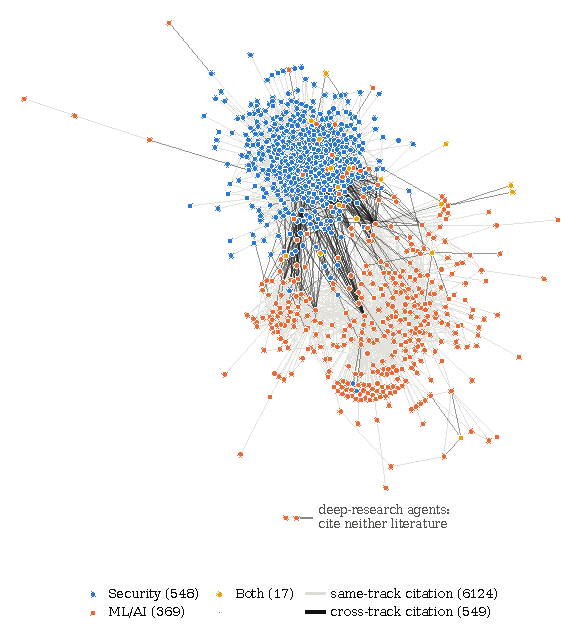
\includegraphics[width=\columnwidth]{figures/fig5_citation_network}
\caption{The corpus as a citation graph: \NNetworkNodes{} papers that cite or are cited
by another included paper, \NNetworkEdges{} edges. Node colour is track. Pale edges are
citations within one literature, dark edges cross between them. The two
communities form separate clusters joined by a narrow band. Note that 8.2\% of
\emph{edges} cross tracks, which is not the same measurement as the per-paper
rates in the text: a paper counts there if it has at least one cross-track
citation anywhere in its reference list. Papers with no resolved citation link to any other
included paper are omitted from the drawing.}
\label{fig:network}
\end{figure}

\subsection{Evaluation}

Citation is a weak test. A paper can cite a neighbouring literature in one line
of related work and ignore it everywhere else. The stronger test is whether a
defense is ever \emph{evaluated} against a mechanism from the other track.

Of the confirmed defense-by-mechanism test pairs in our coverage matrix,
\textbf{230 of 232 (99.1\%) stay inside a single track. Two cross it, and only
one is a genuine cross-community test.}

This is roughly an order of magnitude worse than the citation gap. The two
literatures cite each other rarely. They evaluate against each other's problems
almost never.

\subsection{What the split costs}

Three consequences follow, and all three are visible in the numbers.

\textbf{Named problems go unanswered.} \NMechUncovered{} of
\NMechanismsBench{} named mechanisms (\PctMechUncovered{}\%) have no defense
ever evaluated against them. Among named injection variants,
\NInjUncovered{} of \NInjVariants{} have zero tested defenses, while the single umbrella entry "indirect
prompt injection" absorbs 76 pairs, which is 32.6\% of all pairs in the matrix.
The field tests heavily against a category and lightly against its members.

\textbf{Effort concentrates where it is already dense.} The incidental half has
4.6 defenses per failure mode and the adversarial half has 1.4 per attack, as
Section~\ref{sec:taxonomy} reports. A community that does not read the other
one cannot see that it is crowding.

\textbf{Methods are adopted without a worst-case check.} \PctOneThreatModel{}\% of defenses were
validated against one threat model. For the \NIncOnly{} validated only on incidental
benchmarks, no one has asked what an adversary does to them. That question is
what Section~\ref{sec:experiments} answers for a sample of them.

\section{What has been tested against what}
\label{sec:coverage}

\subsection{Building the matrix}

We cross-reference the mechanism census against the defense census and record a
pair only when a paper \emph{evaluated} the defense against that named
mechanism. A claim that a defense addresses a problem is not a pair. We mined
each defense paper's baselines, results and technical description for named
mechanisms actually tested against, and favoured false negatives over false
positives.

Reading only defense papers biases the matrix, because a defense paper chooses
which attacks to run. We therefore added a reverse pass over the \emph{attack}
papers, which report a defense losing in a way no defense paper will. The
reverse scan covered the full mechanism registry and recovered 54 pairs that
the defense-side scan had missed, 12 of them against mechanisms that had no
tested defense at all. The final matrix holds \textbf{\NPairsComposite{}
confirmed pairs}.\footnote{Three denominators appear in this paper and we keep them
distinct. 332 is the full matrix, including the supplementary passes and the
reverse scan. 233 is the base matrix from defense-paper reads alone. 232 is the
subset for which we could also determine the reporting side and the reported
outcome, which is the base used in Section~\ref{sec:whoran} and for the
same-track rate in Section~\ref{sec:literatures}. All three are produced by
one script from the registries, and \NPairsComposite{} supersedes the 332
published in RQ5, which predates reverse-scan pass 3.}

\subsection{The matrix is sparse, and sparse in a specific way}

\begin{itemize}
\item \textbf{\NDefMatchedFull{} of \NDefenses{} defenses
  (\PctDefMatched{}\%)} have at least one confirmed test against a named
  mechanism. The rest were not evaluated against anything our registry
  recognizes as a distinct named technique. \emph{That is not the same as
  untested}, and the distinction matters enough that we audited it
  separately: see below.
\item \textbf{\NMechUncovered{} of \NMechanismsBench{} mechanisms
  (\PctMechUncovered{}\%) have zero defenses} evaluated against them.
\item \textbf{\NDefMatchedFull{} defenses appear in at least one pair, and
  \NDefOneFull{} of them (\PctDefOneFull{}\%) appear in exactly one.}
  Thirty-four appear in two, 23 in three, and \NDefFourPlus{} in four or
  more. The most cross-tested defense appears in \NDefCeiling{} pairs.
\end{itemize}

The third point needs care, because the answer depends on which evidence you
count, and the difference is itself a finding.

\textbf{Counting only what defense papers report, there is essentially no
generalist defense.} In the base matrix, built from defense-paper reads alone,
\NDefOneBase{} of \NDefMatchedBase{} matched defenses (\PctDefOneBase{}\%)
were tested against exactly one mechanism,
and cross-mechanism testing tops out at three mechanisms, twice, in a corpus
of \NCorpus{} papers.

\textbf{Adding the attack-paper scan raises the ceiling, but changes what
breadth means.} On the full pair set the most-tested defense appears against
\NDefCeiling{} distinct named attacks, and \NDefFourPlus{} defenses appear
against four or more. Of the pairs belonging to those \NDefFourPlus{}, 46\% were contributed by attack papers rather
than by the defenses' own evaluations. For the single broadest case, SecAlign,
seven of its eight pairs come from attack papers. Its breadth is not evidence
that it was evaluated widely by its authors. It is evidence that attackers
chose it as a target, and by Table~\ref{tab:whoran} those are pairs the defense
lost.

So the two readings do not conflict. Defense authors test narrowly. The
defenses that look broadly tested are mostly the ones that attracted attackers.
Either way, a claim that a method provides broad protection against context
poisoning is, on the current evidence, untested rather than wrong.

\subsection{How much of the gap is the field, and how much is us}

A coverage matrix measures resolution against a named registry. It is easy to
read the complement as "never tested", and that reading is wrong. A defense
paper that runs on AgentDojo without naming which injection it used is
evaluated adversarially. It is not a (defense, mechanism) pair, because
expanding a benchmark to all of its constituent attacks would manufacture
coverage, and we refuse that expansion throughout. It is not untested either.

We therefore audited the \NDefenses{} defenses against a coarser question: did
anyone run any comparison at all? \textbf{14 defenses (2.7\%) report no
baseline comparison of any kind.} Each of the 14 was confirmed by hand. Their
own evaluation sections say so: "No comparison against existing forensic or
IPI-detection methods is reported", "No empirical baselines. The comparison is
conceptual", "authors explicitly acknowledge the absence of a baseline method
comparison". One proposes a defense with no implementation at all.

So the honest statement of the gap is narrower than the matrix alone suggests.
\textbf{Most defenses were evaluated. What most of them were not evaluated
against is a second named mechanism, and what almost none were evaluated
against is the other community's threat model} (Section~\ref{sec:literatures}).
A keyword audit of the remaining evaluation descriptions is reported in the
artifact, but we do not quote its middle categories here: hand-checking showed
roughly half of its flagged cases were classifier misses rather than real
ones, which is the same claim-versus-evidence error this paper is about and is
not a basis for a number in a systematization.

\subsection{The result depends on who ran the experiment}
\label{sec:whoran}

The reverse scan makes a second measurement possible. For every pair we also
record which side of the field reported it, and what outcome was reported.

\begin{figure}[t]
\centering
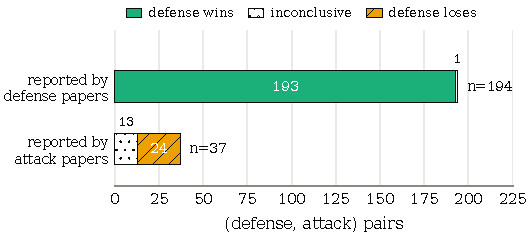
\includegraphics[width=\columnwidth]{figures/fig3_who_reports}
\caption{The same defenses and the same attacks, reported by the two sides of
the field. A defense paper reports its defense winning in 193 of 194 pairs. An
attack paper reports the defense winning in none of 37.}
\label{fig:whoreports}
\end{figure}

\begin{table}[t]
\caption{Reported outcome of a (defense, attack) pair, by who reported it.
Same defenses. Same attacks. Opposite verdicts.}
\label{tab:whoran}
\small
\begin{tabular}{@{}lrrr@{}}
\toprule
\textbf{Reported by} & \textbf{Pairs} & \textbf{Defense wins} &
\textbf{Defense loses} \\
\midrule
defense papers & 194 & \textbf{193} & 0 \\
attack papers  &  37 & \textbf{0}   & 24 \\
\bottomrule
\end{tabular}
\end{table}

\textbf{When a defense paper reports a pair, the defense wins 193 times out of
194. When an attack paper reports a pair, the defense wins zero times out of
37.} The remaining attack-paper pairs are inconclusive rather than wins.

We are not claiming misconduct. Each side runs the experiment it has reason to
run, under conditions it chose, and publishes what it finds. An attack paper
exists because its attack works, so it selects defenses its attack defeats. A
defense paper exists because its defense works, so it selects attacks its
defense stops. Both selections are rational and both are published in good
faith.

The consequence is still that \textbf{the published outcome of a
(defense, attack) pair is close to fully determined by which side wrote the
paper}, and the two sides rarely write about the same pairs. A reader
assembling a picture of "what works" from defense papers alone, which is what
the citation data in Section~\ref{sec:literatures} suggests most readers do,
will assemble one in which defenses essentially always work.

This is the strongest argument we can make for the experiments that follow.
When a literature's reported outcomes are this strongly conditioned on
authorship, the only way to learn what a defense does against an attack it was
not built for is to run it.

\section{The platform}
\label{sec:experiments}

Section~\ref{sec:emptycell} ends at a cell nobody has filled. This section
describes the instrument we built to fill it. It is one harness. It runs a
published defense against a published attack under one protocol, with the
controls fixed before any run. The next two sections report what it
produced, and together they answer RQ2.

\subsection{Pair selection}

The taxonomy picks the (defense, attack) pair under two conditions. The defense and
the attack must occupy the same taxonomy cell, which means the content enters
through the same channel and causes the same consequence. And no paper in the
corpus may report having run them together. A defense that repairs quiet answer corruption arriving through retrieval
ought to apply to an attack that arrives the same way and does the same
damage. The taxonomy says so. Nobody had checked.

We are not proposing new defenses. Every method we run is published, and
every attack we run is published. The contribution is the pairing.

\subsection{The reconstruction standard}

The taxonomy decides which pairs we run, and this rule decides what counts as
running one. Every number we report comes from running a defense's own released code and
weights. We never cite a paper's reported numbers as evidence about that
paper's method. Where a harness had to be adapted to our data, we adapted the
harness and left the method and the evaluation rubric untouched. Where an
author's rubric and ours differed, we used the author's.

The standard cost us coverage. Several defenses could not be evaluated at
all, for reasons that lie in what their artifacts ship rather than in what
their methods do, and we record those as roadblocks rather than as failures
of the method.

\subsection{Pre-registered experimental rules}

Released code is not enough on its own. A negative result is easy to produce
by accident, so four rules guard against that, and we fixed all four before
any run.

\textbf{The control fires first.} A defense that is broken in our hands
tells us nothing about transfer, so before any transfer number we check that
the method still does, in a clean context, what its authors say it does. The check is directional, and it is set per method, because no two papers
claim the same quantity. ParamMute~\cite{huang-2025-parammute} reports a gain in context
recall, not in accuracy. CK-PLUG~\cite{bi-2025-parameters} claims no accuracy gain at all: its
contribution is a knob that moves memorization rate while accuracy is held,
so its control fires on that rate instead. ACD~\cite{kim-2024-adaptive} states its improvement
without a figure. SCR's~\cite{huang-2024-trust} own authors report it underperforming their
baseline on Llama-3-8B, the model we run it on, so on this model there is no
published gain to reproduce, and agreement with them means moving the same
way they report. For each method, we therefore check the direction of the change, on the metric
that paper uses for the model it used. We record which quantity each
control was read on. Where no comparable published figure
exists, we say so rather than manufacture a threshold.


\textbf{The attack works first.} If the attack does not degrade the undefended
arm in the same run, the defended arm means nothing. Every result below is
reported next to an undefended arm measured on the same items at the same doses
with the same scorer.

\textbf{Effects are gated on a minimum detectable change.} For each run we
compute the smallest difference detectable at the given sample size with
$\alpha = .05$ and power $.80$. Differences below it are reported as "no
resolvable effect", never as "no effect". This matters because several
published claims in this area rest on differences that a run of their size
cannot resolve.

\textbf{Attacks are not adapted to the defenses they meet.} An attack that is not built for a defense and
defeats it anyway is a lower bound on attack strength: if the
cheapest payload wins, an adapted one also wins. So non-adaptive evaluation is
conservative for a claim that a defense fails, and invalid for a claim that one
holds. Every failure we report is of the first kind. The single resistance
result we report is of the second, and we test it adaptively rather than
asserting it.

Predictions were written into the runner scripts and committed to version
control \emph{before} each run, and they ship with the artifact.

\subsection{What we ran}
\label{sec:whatweran}

Every pair we ran is two choices: which literature the defense came from,
and which literature the failure came from. That makes four boxes, and they
do not ask the same question.

Two boxes are home ground. A method meets the kind of failure its own authors
built it for, so nothing there tests transfer. These are where the first rule
above is satisfied, and they hold \NCampSecDefSecMech{} and
\NCampSafDefSafetyMech{} of our \NCampaignPairs{} pairs.

The other two boxes are crossings, and each asks its own question.

The first crossing puts an adversary in front of a method built for honest
error. These are methods for a context that is merely wrong --- out of date,
or contradicted by what the model already believes --- and the question is
what they do when someone chose the wrong text on purpose. That is most of
what we ran, \NCampSafDefSecMech{} pairs.

The second crossing runs the other way. It gives a method built against an
adversary a failure nobody wrote. The question is whether such a method needs
an attacker to earn its place, or whether it helps whenever the context stops
supporting the right answer. This is the smaller side,
\NCampSecDefSafetyMech{} pairs.

Inside each crossing the pairs vary along one axis, and it is a different
axis in each. Going one way, what changes is how much the attacker controls:
a passage optimized against the retriever, a fluent sentence asserting a
chosen answer, a passage that steers behavior rather than the answer, and a
passage optimized against the defense itself. Going the other way, what
changes is whether anything arrives at all: text that reaches the window and
should not be believed although no one wrote it to deceive, against a window
whose contents all deserve belief and which stops working because there is
simply more of everything.

The four boxes are not spread evenly across the two rigs the campaign runs
on. The retrieval cell holds all four. The agent cell holds one: every
technique in it is a prompt-injection defense and every attack an AgentDojo
injection, so all \NAgentPairs{} of its pairs are a security defense meeting
a security mechanism. Every crossing we report is therefore a retrieval-cell
result, and the agent cell tests no transfer at all.

The two crossings together are \NCampCrossPairs{} of \NCampaignPairs{}
pairs, \PctCampCross{}\% against the \PctCrossCommunity{}\% the
literature manages,
and \NRagImplSafety{} of our \NRagImpl{} retrieval defense implementations
are knowledge-conflict methods meeting an attack. That is the literature's
empty column, populated. Counted at registry-name level,
\NRagPairsNovel{} of \NRagPairsKeyed{} pairs are absent from the
\NPairsComposite{} the literature reports, and the two that are not are the
home-ground pairs their own papers already ran.

The retrieval cell pairs defenses built for knowledge conflict against
attacks built to poison a retrieval corpus. The victim model is
Llama-3-8B-Instruct~\cite{grattafiori-2024-llama3} or Mistral-7B-Instruct~\cite{jiang-2023-mistral}, depending on what each defense
released. The data is CoConflictQA~\cite{huang-2025-parammute} over Natural Questions, and open Natural
Questions for the attacks that need a retrieval pool.

Those defenses turn the same dial. ACD decodes from the no-context
distribution and pulls it toward the with-context one by a weight computed
from entropy. CK-PLUG interpolates the two
distributions under a single parameter. ParamMute
suppresses the feed-forward layers that carry parametric memory, forcing the
model onto the retrieved text. SpARE~\cite{zhao-2024-steering} and
SHIFT~\cite{li-2026-shift} steer along a context-faithfulness direction in
activation space. COIECD detects a conflict
between the two sources and pushes toward the context.
SCR makes the same trade through prompting rather
than decoding. Each changes \emph{how much} the model leans on retrieved
text. None asks \emph{which} retrieved text deserves trust.

The agent cell pairs ingestion-stage and execution-stage defense
techniques against prompt-injection attacks inside the AgentDojo banking
suite~\cite{debenedetti-2024-agentdojo}, with a Qwen2.5-14B-Instruct~\cite{qwen-2024-qwen25} agent.

In total we executed \NCampaignPairs{} distinct (defense, attack) pairs
across \NCampaignImpl{} defense implementations, over \NCampaignEpisodes{}
scored episodes: \NRagPairs{} pairs and \NRagEpisodes{}
episodes in the retrieval cell, \NAgentPairs{} pairs and \NAgentEpisodes{}
episodes in the agent cell.
The two episode counts are not comparable units. An agent episode is a complete
multi-step tool-use trajectory. A retrieval episode is one scored answer.

Every run in this paper used one NVIDIA RTX A6000 with 48\,GB, driver
535.274.02 and CUDA 12.8, under Python 3.10.12, PyTorch 2.10.0 and
\texttt{transformers} 5.5.0. Two defenses cannot use that last version. ACD's
released decoder imports symbols that \texttt{transformers} removed after
4.44, which its own README pins, so it runs in a separate dependency set.
CK-PLUG ships its own 4.49 fork and its README says to install it. We record this
because it is a result as much as a configuration detail. The defenses in a
single cell of this taxonomy cannot share one Python environment. That is the
reproducibility problem of Section~\ref{sec:discussion}, one layer further
down. The released artifact builds each set and verifies it.

\subsection{Datasets}
\label{sec:provenance}

An \textbf{item} is one question, its gold answer, and the context the model
is given to answer it from. Every item in this paper belongs to the authors
of the method or the benchmark we are running. Table~\ref{tab:provenance} lists each source and whose it is. This is deliberate rather than convenient. A defense
evaluated on the distribution it was designed for cannot blame its failure on
an unfamiliar dataset. A result obtained that way is harder to dismiss than
one obtained on data we chose ourselves.

\begin{table}[t]
\centering
\caption{Item sets and payloads, by owner. No item set is ours. Three
payloads come from the attack literature and five are ours, and none of the
five is a new attack: three are edits of a field the benchmark already ships,
and two reuse the item set's own retrieved passages, which is what makes them
controls rather than attacks.}
\label{tab:provenance}
\small
\begin{tabular}{@{}>{\raggedright\arraybackslash}p{0.40\columnwidth}>{\raggedright\arraybackslash}p{0.52\columnwidth}@{}}
\toprule
\textbf{Item set} & \textbf{Released by} \\
\midrule
CoConflictQA~\cite{huang-2025-parammute} over Natural Questions & the ParamMute authors \\
Open Natural Questions~\cite{kwiatkowski-2019-natural}, with its retrieval pool & the RobustRAG authors \\
FaithEval~\cite{ming-2025-faitheval}, SQuAD~\cite{rajpurkar-2016-squad} negatives & the FaithfulRAG~\cite{zhang-2025-faithfulrag} authors \\
AgentDojo banking suite & the AgentDojo authors \\
\midrule
\textbf{Payload} & \textbf{Origin} \\
\midrule
Corpus poisoning & Zhong et al.'s released passage, unmodified \\
PoisonedRAG, BadRAG & The published constructions \\
False evidence & CoConflictQA's own parametric-evidence field \\
Distractor evidence & \textbf{ours}: one substitution into that field \\
Adaptive distractor & \textbf{ours}: the same claim, reshaped against one
defense's rule \\
Gradient distractor & \textbf{ours}: that passage and a suffix optimized
against the same rule \\
Stale document & \textbf{ours}: a real retrieved passage, gold answer
swapped \\
Misretrieval & \textbf{ours}: a real passage, unmodified, retrieved for
another question \\
\bottomrule
\end{tabular}
\end{table}

Every comparison in this paper is between arms measured on the same items.
Rates computed on different item sets are incomparable rather than merely
noisy, so we checked this mechanically rather than by inspection: across
every result registry, no run compares two arms measured on different items.

The one place the item set narrows is the distractor payload, and it narrows
for both arms together. It is defined on \NDistractorItems{} of CoConflictQA's
\NCoConflictItems{} items. An item
qualifies on two conditions. Its remembered answer must appear verbatim in its
own evidence sentence, so that the substitution needs no rewriting. And its
question type and answer magnitude must admit at least three candidate
distractors, so that the planted answer is a plausible example of its kind
rather than an absurdity a reader would dismiss. Every arm in those runs, including the undefended and no-retrieval
arms, is measured on that same subset.

\subsection{Payload classes}
\label{sec:payloadclasses}

The retrieval cell evaluates every item whose context is at most 2000
characters. The cut is on context length alone, never on an outcome, and it
is applied once and then frozen, so every defense and every payload meets the
same items. Its purpose is memory. Contrastive-decoding defenses hold two
forward passes of the model at once, and this keeps the whole cell inside one
card at a batch size every defense can share.

On those items we hold the dosing and the scorer fixed as well, and vary only
the \emph{form} of the planted passage. There are five forms. They differ in
how the passage reads and in what it does to the evidence, and a defense that
behaves differently across them tells us which property it is actually keying
on.

Corpus poisoning~\cite{zhong-2023-poisoning,su-2024-corpus} optimizes a
token sequence to be retrieved for many queries. The resulting passage is
incoherent to a human reader. It attacks by displacing honest documents.

False evidence does the opposite. It plants a fluent, well-formed sentence
that asserts the wrong answer the model itself would have given from memory. It is drawn from
CoConflictQA and reads like an ordinary encyclopaedia sentence. It attacks by
agreeing with the model's prior.

Distractor evidence is that same fluent sentence with one word changed, so
that it asserts a third answer which is neither the truth nor the model's
prior. It is not a stronger attack. It is a measuring instrument, and
Section~\ref{sec:distractor} explains why it was necessary.

An adaptive distractor is the distractor payload again, in whichever surface
form minimizes the quantity one defense's rule measures. A gradient
distractor is that passage with a short optimized suffix appended against the
same quantity (Section~\ref{sec:results2}).

Three of the five are ours, the distractor and its two optimized forms, and
all three are edits of a field that already ships with the benchmark. That field is worth
drawing out. False evidence is the
\texttt{parametric\_evidence} field that ships inside CoConflictQA, the
benchmark the ParamMute authors released themselves. One of the defenses we
break is broken with a field from its own dataset.

\paragraph{Dose, and the one item set that has none.}
The \textbf{dose} is how many of the retrieved passages are planted. It is
the axis every result in this paper is read along, because a defense that
holds against one poisoned passage and fails against five has not failed in
the same way as one that never helped.

We take the dose from the attacks rather than define one. Their released
constructor is parameterised by how many of the top $k$ retrieved passages
it replaces, where it places them and how often the planted sentence repeats
inside its passage. We keep that construction and sweep the one parameter:
$j$ of the top ten, for $j$ in $\{0, 1, 2, 3, 5, 10\}$. Their own default is
$j = 1$, so their setting is one of our points and the rest are further
readings of the same instrument.

One item set has no such axis and we do not give it one. CoConflictQA
supplies a single context passage per item, which either carries the
conflicting claim or does not, and a single passage has no ranked list to
dose. We report it in the two conditions its own authors run, a clean
context and a corrupted one. The two item sets are never combined in one
number.

Every result file also carries a fingerprint of the payload it was produced
with, so a run cannot be read under the wrong attack label.

\section{Results: the context-reliance family under attack}
\label{sec:results}

\subsection{One design rule explains most of what we found}

Stated first, then supported: \textbf{a defense that works by shifting trust
from the model's parameters toward the retrieved text is correct when the text
is merely stale and dangerous when an attacker owns it.}

This family is large. It includes
ParamMute~\cite{huang-2025-parammute}, CK-PLUG~\cite{bi-2025-parameters},
SpARE~\cite{zhao-2024-steering}, COIECD~\cite{yuan-2024-discerning} and
SHIFT~\cite{li-2026-shift}. All were published as fixes for knowledge
conflict, and all were validated against the incidental threat model only. The
family's shared idea is reasonable for the problem it was built for. When a
retrieved document disagrees with the model's memory, the document is usually
newer, so trust the document. The idea becomes a liability the moment the
document is written by an adversary, because the defense instructs the model to
trust the one thing the adversary controls.

\begin{table}[t]
\caption{Context-reliance defenses against corpus poisoning, each read against
its own undefended arm in the same run. "Clean" is the defense's own published
benefit. "Saturation" is 100\% poisoned context. Bold clears that run's
minimum detectable change.}
\label{tab:family}
\small
\begin{tabular}{@{}lrrrr@{}}
\toprule
\textbf{Defense} & \textbf{$n$} & \textbf{mdr} & \textbf{Clean} &
\textbf{Saturation} \\
\midrule
ParamMute & 1409 & 5.3 & \textbf{+9.3} & \textbf{-4.2} \\
CK-PLUG   &  800 & 7.0 & \textbf{-10.1}$^{\dagger}$ & \textbf{-9.9} \\
SpARE     &  500 & 8.9 & \textbf{+14.2} & \textbf{-10.2} \\
COIECD    &  400 & 9.9 & -0.8 & -1.8 \\
\bottomrule
\end{tabular}
\\[2pt]
{\footnotesize $^{\dagger}$CK-PLUG's control fires on memorisation rate rather
than accuracy, so its clean cell reports that metric.}
\end{table}

SpARE is the cleanest case because its control and its conviction are the same
measurement. Steering toward the context is worth \textbf{+14.2\pp} when the
context is honest and costs \textbf{-10.2\pp} when it is attacked. Both ends
clear the 8.9\pp threshold. The sign flips.

ParamMute shows the same shape on a larger sample. Its benefit on clean context
is +9.3\pp. At saturation it is 4.2\pp \emph{below} the undefended model, and
across the full dose range it loses 13.5\pp more accuracy than doing nothing at
all.

CK-PLUG's behaviour is the most extreme we measured, and it appears on a
different metric. Under BadRAG sentiment steering~\cite{xue-2024-badrag}, which
tries to make the model answer in a negative tone, the undefended model adopts
the attacker's framing 0.0\% of the time at every dose. CK-PLUG adopts it
78.2\% of the time with a single poisoned passage out of ten, and 99.0\% at
full dose. The defense does not fail to stop the attack. It carries it.

\begin{figure*}[t]
\centering
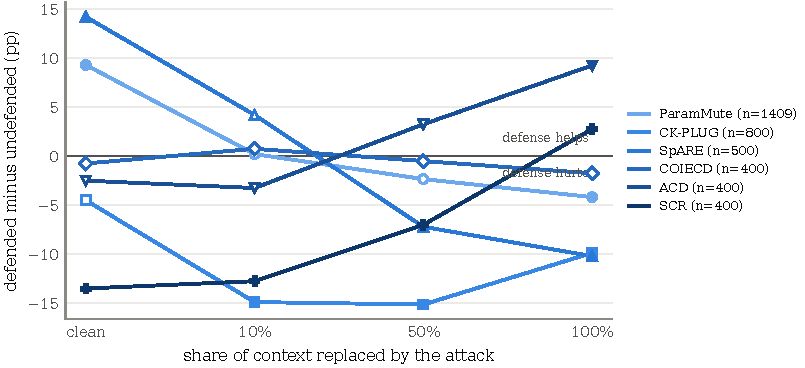
\includegraphics[width=0.82\textwidth]{figures/fig4_dose_response}
\caption{Every retrieval-cell defense against corpus poisoning, measured as the
defended arm minus its own undefended arm in the same run. Zero means the
defense changed nothing. Filled markers are resolvable at $p < .05$ by Fisher's
exact test, hollow are not. Three patterns are visible. SpARE and ParamMute
start above zero and cross it, which is the sign flip. CK-PLUG and SCR sit
below zero almost everywhere, costing accuracy before the attack arrives. ACD
is the only line that rises, and Table~\ref{tab:acd} shows that rise does not
survive a change of payload.}
\label{fig:dose}
\end{figure*}

\subsection{The scope condition}

The rule is not that suppressing parametric memory is always harmful. We can
state when it is.

\textbf{Suppressing the model's prior knowledge hurts only where that prior
knowledge held the right answer.} Against BadRAG's denial-of-service variant,
which makes the model refuse rather than answer wrongly, ParamMute is strongly
protective. With one poisoned passage in ten the undefended model refuses
52.4\% of the time and holds 27.0\% accuracy. ParamMute drops refusal to 0.2\%
and restores accuracy to 57.4\%, within 2.4 points of its own clean baseline.
Across the realistic range of one to five poisoned passages, the undefended
model averages 25.8\% accuracy and ParamMute averages 57.6\%.

The mechanism is the same in both cases. ParamMute suppresses the model's
memory. When memory held the correct answer, that suppression destroys it. When
the attack works by driving the model into refusal, suppressing memory removes
the conflict that triggered the refusal. \textbf{One mechanism, two signs,
selected by whether the memory was right.} We predicted little effect here and
were wrong, which is why the scope condition is in the paper.

\subsection{The payload class decides, not the attack label}

ACD~\cite{kim-2024-adaptive} was the best result in our campaign. It discounts
tokens the context makes uncertain, and against corpus poisoning it is the only
method that both reads a clean document and resists a poisoned one. At
saturation it is \textbf{+9.2\pp} above the undefended arm ($p < 0.0001$) and
on clean context it is \textbf{+53.5\pp} above answering with no document at
all.

We then ran the same defense, same items, same doses, against false evidence.

\begin{table}[t]
\caption{ACD against two payload classes, $n=400$, mdr 9.9\pp. The defense is
unchanged. Only the form of the planted passage differs.}
\label{tab:acd}
\small
\begin{tabular}{@{}lrr@{}}
\toprule
\textbf{Comparison at saturation} & \textbf{Corpus poisoning} &
\textbf{False evidence} \\
\midrule
vs.\ undefended  & \textbf{+9.2} ($p{<}0.0001$) & +3.0 ($p{=}0.059$) \\
vs.\ no retrieval & +0.5 ($p{=}0.91$) & \textbf{-4.0} ($p{=}0.0499$) \\
\bottomrule
\end{tabular}
\end{table}

\textbf{The protection collapses.} Against the incoherent payload, ACD restores
the no-retrieval floor exactly. Against the fluent payload it ends up
resolvably \emph{below} that floor: the defended model does worse than a model
given no document at all.

The reason is visible in the method. ACD keys on the uncertainty a passage
induces. An optimized token string is incoherent and raises uncertainty, so ACD
discounts it. A fluent sentence asserting a plausible wrong answer lowers
uncertainty, so ACD trusts it more.

This has a practical consequence. \textbf{The cheaper and more natural-looking
attack is the stronger one.} For COIECD's undefended arm, false evidence cuts
accuracy roughly twice as far as gradient-optimized corpus poisoning at every
dose, falling to 15.2\% at 10\% dose against 26.5\% for corpus poisoning. The
field's attention to optimized adversarial passages is not matched by their
effectiveness.

\subsection{Two payloads, three defenses, three outcomes}
\label{sec:payloads}

ACD is not the only method whose behaviour depends on the form of the planted
passage. We ran the three context-reliance defenses whose corpus-poisoning
results are already in Table~\ref{tab:family} against false evidence as well,
each against its own undefended arm over the same items at the same doses.
Predictions for all three were committed to version control before any of them
ran.

\begin{table}[t]
\caption{The same three defenses against two payload classes. Excess damage is
the defended arm's clean-to-saturation collapse minus the same collapse in its
own undefended arm; positive means the defense lost more accuracy than doing
nothing would have.}
\label{tab:payloads}
\small
\begin{tabular}{@{}lrrr@{}}
\toprule
\textbf{Defense} & \textbf{$n$} & \textbf{Corpus poisoning} &
\textbf{False evidence} \\
\midrule
ParamMute & 1409 & \textbf{+13.5} & \textbf{+12.3} \\
CK-PLUG   &  800 & \textbf{+5.4}  & +0.4 \\
COIECD    &  400 & +1.0           & -1.2 \\
\bottomrule
\end{tabular}
\end{table}

\textbf{ParamMute is harmful against both, and the way it fails is the
finding.} A defense worth +9.7\pp on honest context costs 12 to 13 points more
than doing nothing once an adversary writes the context, and it does not matter
whether the adversary writes gibberish or prose. What does change is how well
ParamMute does its own job. Its suppression of the wrong parametric answer
falls from \textbf{-42.5\pp} under corpus poisoning to \textbf{-8.8\pp} under
false evidence. The reason is structural. Under corpus poisoning the wrong
answer has one source, the model's memory, so inhibiting memory removes it.
Under false evidence it has two, memory and the planted passage, and ParamMute
touches only one of them. \textbf{The attack duplicated the answer into the
channel the defense does not operate on.}

\textbf{CK-PLUG is harmful against one payload and flat against the other}, and
the shape matters more than the sign. Under corpus poisoning its cost grows
with the attack: -4.5\pp on clean context, then -14.9 and -15.1 once poison is
present. Under false evidence it is a constant offset of about -4.4\pp at every
dose including the clean one, and no cell clears the 7.0\pp threshold. CK-PLUG
pays a fixed price for being switched on; corpus poisoning amplifies that price
and false evidence does not.

\textbf{COIECD is inert against both.} Eight comparisons, largest 1.8\pp
against a 9.9\pp threshold, no $p$ below 0.20. Its memorisation-rate
suppression does shrink roughly threefold under false evidence, which is what
an entropy constraint should do when the planted passage agrees with the prior
rather than contradicting it, but that signal sits below threshold and we
record it as directional rather than as a result.

\subsection{A comparison we decline to make}

The three results invite a ranking across payload classes, and we committed in
advance to treating one as a falsifier: if any defense did \emph{better}
against false evidence than against corpus poisoning, then "these defenses fail
because they trust the context" would not be the mechanism. CK-PLUG does, at
+0.4\pp against +5.4\pp.

We do not think that reading survives inspection, and we say so rather than
quietly dropping the test. The two payloads are not equally strong on the
undefended arm. False evidence is roughly twice as damaging at every dose: for
CK-PLUG's undefended arm, 23.0\% against 39.2\% at 10\% dose, and for COIECD's,
15.2\% against 26.5\%. Excess damage is a difference of two collapses, and when
the undefended arm has already collapsed there is less room left for a defense
to make things worse.

\textbf{Excess-damage comparisons across payload classes are therefore
confounded by attack strength and should not be read as a ranking.} Within a
payload, against the control measured beside it in the same run, every
comparison in this section stands. We state the limit because the alternative
is to report a falsifier as passed when the instrument cannot support it.

One measurement limit belongs here for the same reason. Under false evidence
the planted passage asserts the same string the model would have recalled, so
the parametric-answer rate cannot distinguish a model that remembered from one
that copied. They produce identical output. That is the attack's design rather
than a flaw in the metric, and it means ParamMute's residual 58.8\% cannot be
split between the two paths. An arm that plants the \emph{gold} answer instead
would separate them.

\subsection{Asking the model to judge the document}

SCR~\cite{huang-2024-trust} is the only method we ran whose design anticipates
an adversary. It shows the model its own no-context answer, the document, and
the answer the document supports, and asks the model to judge which to believe.

It does help at saturation, +2.8\pp over the undefended arm ($p = 0.025$), and
it does genuinely read the document, scoring 41.2\pp above no-retrieval on
clean context. \textbf{It pays 13.5 points on clean data to buy that 2.8.} The
cost is resolvable at every dose below saturation and is roughly five times the
benefit. A defense deployed permanently and attacked occasionally is a poor
trade at that exchange rate.

SCR's parametric-answer rate climbs 22.8, 33.8, 35.8, 52.5 across the dose
range, converging on the closed-book rate of 55.8. Both SCR and ACD slide from
the document toward memory as the attack grows. SCR simply destroys more
correct answers on the way.

\section{Recommendations}
\label{sec:discussion}

\subsection{Controls both communities should report}

Section~\ref{sec:results2} reports three results that read the other way
without the arm beside them. None of the three arms is expensive. None is
currently standard. We propose all three as reporting requirements.

\textbf{Report a no-retrieval arm.} Any defense that modifies how a model uses
retrieved context must report what the same model scores with no retrieved
context at all. Without it, a defense that has stopped reading the document is
indistinguishable from a defense that has learned to resist a poisoned one.
This is one extra arm and it costs one extra pass over the data.

\textbf{Report the abstention rate, not only accuracy.} A method that converts
confident wrong answers into refusals has done something valuable and will
score as inert on accuracy. In an agent setting, where a wrong answer becomes a
wrong action, that difference is the whole point. Reporting where the
probability mass went, rather than only whether it landed on the gold answer,
costs nothing beyond classifying the generations already produced.

\textbf{Report at least two base models.} Holding defense and attack fixed and
changing only the model changed an effect's magnitude, its existence, and once
its sign. A single-model result in this area should be read as a
model-specific result until shown otherwise.

\subsection{Conventions for measurable transfer}

\textbf{State the regime the evaluation actually covers.} Our defense
census codes each method by what its own paper evaluated, and
\PctOneRegime{}\% cover one regime. Many of those papers describe their
contribution in terms broad enough to imply the other. One required sentence
would close this. Name the regime the experiments cover. A reader of the
paper, and the maintainer of a system, then sees the gap without reading the
appendix.

\textbf{Gate claims on a detectability threshold.} Reporting a difference
without the smallest difference the experiment could have detected makes "no
effect" and "we could not tell" look identical. We computed this for every run
and several of our own results moved from the first category to the second.

\textbf{Say whether the attack was adapted to the defense.} A defense that
holds against an attack built for a different target has been shown to resist
that attack and nothing more. The asymmetry matters and papers rarely state it.
Non-adaptive evaluation is conservative evidence for a failure. It is no
evidence at all for a guarantee. Every published evaluation of a
context-reliance defense in our corpus is non-adaptive. We built an adaptive
payload against the one method that had resisted, and
\PctAcdRemovedGradient{}\% of its protection
went (Section~\ref{sec:adaptive}). One sentence naming whether the
attacker knew the defense would let a reader tell which kind of claim they are
reading.

\textbf{Compose across the boundary, and measure the composition.}
Section~\ref{sec:parallel} shows the two communities defending different
stages of one pipeline, and Section~\ref{sec:results} shows the reasoning
stage failing on its own once an adversary writes the input. The obvious
next move is to put an ingestion-stage filter in front of a
reasoning-stage method and see whether the pair holds where each half does
not. We do not know that it works. Nothing in this paper tests a composed
defense, and a filter that passes a fluent falsehood leaves the reasoning
stage exactly where our results find it. That is the point: the experiment
is cheap, both halves are published with released code, and no paper in
\NCorpus{} has run it.

\subsection{Artifacts}

The reconstruction standard made artifact quality measurable as a side effect.
Among the best-cited untested defenses in the cell we studied, two name
empty repositories. Two more ship code without the trained weights it needs.
One runs. Two further execution-stage defenses do not
run reliably on any freely-available open-weight model.

We note this without blame. Releasing a working artifact is harder than it
looks and is rarely rewarded. But the coverage gap this paper measures is
partly an artifact gap. A defense nobody else can run is a defense nobody else
will test. \PctDefUnmatched{}\% of the defenses in our census have no
confirmed test against any named mechanism.

\subsection{Implications for deployment}

Three practical points follow from the results.

Consider a system that uses a knowledge-conflict method to improve answer
quality, and that also retrieves from a corpus an outsider can write to. The
method then operates outside its validated regime. Our measurements say it
is more likely to increase damage than to reduce it.

A defense that holds against an optimized adversarial passage may fail against
a fluent sentence that simply asserts a plausible falsehood. In our
measurements no defense resisted both. The fluent attack is cheaper to produce. It needs no
gradient access and no surrogate retriever, and it does roughly twice the
damage to an undefended model at every dose. Evaluations built only around
optimized payloads overstate protection. Do not call a defense tested on one
payload class robust to context poisoning.

Finally, the channel matters more than the method name. Supply-chain,
cross-modal and tool-metadata have fewer than one named defense per named
mechanism. If an agent accepts third-party components or machine-readable tool
descriptions, almost nothing published defends that route.

\section{Threats to validity}
\label{sec:threats}

\textbf{Extraction error.} The corpus coding was produced by an LLM-assisted
extraction pass over \NCorpus{} papers and \NCodedFields{} coded fields. Every count in
Sections~\ref{sec:taxonomy} to~\ref{sec:coverage} depends on it. We verified it
with human readers against the original PDFs, in full for the fields that carry
the headline claims and on a random sample for the rest, and we report
inter-rater agreement rather than assuming it. Residual error remains possible
in the sampled fields.

\textbf{Track assignment.} The cross-citation rates depend on classifying every
cited paper into a track. That classification is automated over the full
discovery pool. A systematic bias in it would move the rates. We regard the
direction of the finding as safe, because the gap between \PctSecCitesML{}\% citation and
\PctSameTrack{}\% same-track evaluation is far larger than any plausible classification
error, but the exact rates should be read as estimates.

\textbf{Registry granularity.} What counts as one named mechanism is a
judgement. "Indirect prompt injection" is one registry entry and absorbs 32.6\%
of all tested pairs, while 38 of 52 named injection variants have none. A
coarser registry would make coverage look better and a finer one would make it
look worse. We chose the granularity the papers themselves use, which is the
name each paper gives its own contribution.

\textbf{Who-reports-what is observational.} Section~\ref{sec:whoran} reports a
very strong association between authorship and outcome. It is not a controlled
comparison. The two sides largely write about different pairs, so the
association partly reflects selection of which pair to run, which is exactly
our interpretation, rather than differing conduct on the same pair.

\textbf{The campaign is a sample, not a census.} We ran \NCampaignPairs{} pairs out of a space
of thousands. They were selected by the taxonomy rather than at random, biased
toward pairs where both artifacts run. Defenses whose artifacts do not run are
absent, and nothing here says whether they transfer.

\textbf{Attacks are non-adaptive, with one exception.} This is the criticism
that invalidated DEEPSEC's defense rankings~\cite{carlini-2019-critique} and
we inherit it by design rather than by oversight. Its direction is not
symmetric: an attack not built for a defense that defeats it anyway bounds
attack strength from below, so our failure results are conservative, while a
resistance result drawn the same way is not evidence of robustness.
Section~\ref{sec:adaptive} tests the one resistance result we report. Every
other defense in the campaign would need the same treatment before any claim
that it holds.

\textbf{Variance is argued, not measured.} We use greedy decoding throughout,
so a rerun reproduces exactly, and we report Wilson intervals and a
detectability threshold on every effect. We have not demonstrated that
determinism by rerunning a cell end to end, and we have no multi-seed study of
sensitivity to item order or few-shot choice.

\textbf{Single dataset per cell.} The retrieval cell runs on CoConflictQA and
open Natural Questions. The dosing model, which replaces a fraction of context
with planted passages, is a simplification of a real retrieval pipeline under
attack. It holds the retriever fixed, so it measures what the generator does
with poisoned context rather than how hard the context is to poison.

\textbf{Model coverage.} Most retrieval-cell results use Llama-3-8B-Instruct,
with Mistral-7B-Instruct where a defense required it. Our own model control
shows this is a real limitation: changing the model changed outcomes. The
results should be read as holding for models of this class and size, and the
model control is reported rather than hidden for that reason.

\textbf{Scorer.} We reuse each defense's own evaluation rubric where one
exists, and a shared recall-based rubric across the retrieval cell. Recall
against a gold string rewards a model that produces the right tokens for the
wrong reason. We report the parametric-answer rate and abstention rate
alongside it so that the failure modes stay visible.

\section{Related systematizations}
\label{sec:related}

Several recent systematizations cover parts of this space. Work on the agent
attack surface enumerates attack classes against tool-using systems, and work
on the prompt-injection landscape codes injection papers into structured
comparison tables by method, surface, victim goal and capability. Both are
careful and both are confined to the security literature. Surveys on the
machine learning side cover knowledge conflict, long-context degradation and
retrieval quality, and are likewise confined to their own literature.

Our contribution is not a better enumeration of either side. It is that one
search protocol, one screening pass and one taxonomy are applied to both, which
is what makes the distance between them measurable. A systematization drawn
from one literature cannot report that 9 papers in 10 do not cite the other, or
that 99.1\% of tested pairs stay inside one track, because the other track is
not in its corpus.

The second difference is that we execute. Existing systematizations in this
space report what papers claim their methods achieve. Section~\ref{sec:whoran}
is our reason for not doing that: in this field the reported outcome of a
(defense, attack) pair is close to determined by which side of the community
wrote the paper. A systematization that aggregates those reports inherits that
bias. Running the artifacts is the only way we found to avoid it.

\section{Conclusion and future work}
\label{sec:conclusion}

Two research communities study one failure. An LLM agent reads content it
should not trust, and it cannot tell which content that is. The security
community calls the content an attack and builds defenses. The machine learning
community calls it a mechanism and builds fixes. We placed 984 papers from both
sides into one taxonomy of channel, intent and consequence, and found that the
separation is measurable: about one paper in ten cites the other side, 14 of
529 defenses were validated against both threat models, and 99.1\% of tested
defense-mechanism pairs stay inside a single track.

We then used the taxonomy to find pairs that should have been run and were not,
and ran 81 of them on the authors' released artifacts. The central finding is
that a popular family of fixes, those that repair accidental context failure by
shifting trust from the model's parameters toward the retrieved text, becomes a
liability under deliberate attack, for the reason that is written into its own
design. The finding has a measured scope condition and a counterexample, so it
is a design error rather than a law.

A second result cuts across the first. Protection depends on the \emph{form}
of the planted passage, not only on whether an attacker is present. Running the
same defenses against an optimized adversarial passage and against a fluent
sentence that asserts a plausible falsehood gives different answers, and the
one defense that resists the first falls below a no-retrieval baseline against
the second. The fluent payload needs no gradient access and no surrogate
retriever, and it damages an undefended model roughly twice as hard. An
evaluation built only around optimized payloads overstates how well a system
holds up.

\paragraph{Future work.}
Four directions follow directly.

\textbf{Close the supply-chain and cross-modal gaps.} These channels have fewer
than one named defense per named mechanism and are the routes by which agents
accept third-party capability. They are the clearest place to build rather than
to measure.

\textbf{Separate the intervention-point finding from its confound.} Our case
studies suggest that whether a defense generalizes tracks where in the pipeline
it intervenes. The ingestion defenses that generalize are also the ones whose
harnesses model a text-classification victim, while the execution defenses we
could not evaluate are the agent-shaped ones. Running all three intervention
points inside one agent harness would resolve this, and that work is in
progress.

\textbf{Separate recall from copying.} Under false evidence, the planted
passage asserts the same string the model would have recalled, so our
parametric-answer metric cannot distinguish a model that remembered from a
model that copied. An arm that plants the gold answer instead would separate
them and would sharpen the mechanism claim in Section~\ref{sec:results}.

\textbf{Build the missing evaluation.} The deepest problem this paper documents
is not any single defense. It is that the field's reported outcomes are
conditioned on who ran the experiment, and that nothing in current practice
corrects for it. A shared benchmark that pairs defenses with attacks selected
by a taxonomy rather than by either author would make transfer a measured
property rather than an assumed one.


\bibliographystyle{ACM-Reference-Format}
\bibliography{refs}

\end{document}
